\appendix
\section{Appendix}
\subsection{Example generation of one $X_{t}$~\eqref{eq:Xt} for Barrier options}
\begin{table}[ht]
	\centering
	\begin{lstlisting}
	import pandas as pd
	import numpy as np
	from itertools import product
	
	s, r, g = 5785, 0.040569, 0.01283
	kappa, theta, rho, eta, v0 = 3.676912, 0.255154, -1.0, 0.917628, 0.012088
	K = np.linspace(s*0.8,s*1.2,3,dtype=int)
	T = [30,60]
	B = np.linspace(s*0.5,s*1.2,4,dtype=int)
	R = [0]
	W = ['call','put']
	outin = ['Out','In']
	
	Xt = pd.DataFrame(
		product(
			[s],[r],[g],[kappa],[theta],[rho],[eta],[v0],
			K,B,R,T,W,outin
		),
		columns=['spot_price', 'risk_free_rate', 'dividend_rate', 'kappa', 'theta', 'rho', 'eta', 'v0', 'strike_price', 'barrier', 'rebate', 'days_to_maturity', 'w','outin']
	)
	Xt['updown'] = Xt.apply(lambda row: 'Down' if row['barrier'] < row['spot_price'] else 'Up', axis=1)
	Xt['barrier_type_name'] = Xt['updown']+Xt['outin']
	Xt = Xt.drop(columns=['updown','outin'])
	\end{lstlisting}
\end{table}
The above is an example generation of one $X_{t}$~\eqref{eq:Xt} in python, with $H_{t}$~\eqref{eq:Ht} defined as:
\begin{equation}
	\begin{aligned}
	H_{t}^{\text{Barrier}} = \{ \inlinecode{[s]}, \inlinecode{[r]}, \inlinecode{[g]}, \inlinecode{[kappa]}, \inlinecode{[theta]}, \inlinecode{[rho]}, \inlinecode{[eta]}, \inlinecode{[v0]}, \\ \inlinecode{K},  \inlinecode{T}, \inlinecode{B}, \inlinecode{R}, \inlinecode{W}, \inlinecode{outin}\ \}
	\label{eq:barrierHt}
	\end{aligned}
\end{equation}
where $X_{t}$ is stored in \inlinecode{Xt}, which is a pandas \inlinecode{DataFrame} containing the Cartesian \inlinecode{product} of all elements in $H_{t}^{\text{Barrier}}$~\eqref{eq:barrierHt}: \\
\begin{table}[ht]
	\centering
	\resizebox{\textwidth}{!}{
		\begin{tabular}{lllllllllllllllll}
			\toprule
			& $S$ & $r$ & $g$ & $\kappa$ & $\theta$ & $\rho$ & $\eta$ & $v$ & $K$ & $B$ & $R$ & $T$ & $D^{\text{call/put}}$ & $D^{\text{barrier type}}$ & $y$ & cpu time \\
			\midrule
			0 & 5785 & 0.040569 & 0.012830 & 3.676912 & 0.255154 & -1 & 0.917628 & 0.012088 & 4628 & 2892 & 0 & 30 & call & DownOut & 1167.582527 & 0.038519 \\
			1 & 5785 & 0.040569 & 0.012830 & 3.676912 & 0.255154 & -1 & 0.917628 & 0.012088 & 4628 & 2892 & 0 & 30 & call & DownIn & 0.639513 & 0.075544 \\
			2 & 5785 & 0.040569 & 0.012830 & 3.676912 & 0.255154 & -1 & 0.917628 & 0.012088 & 4628 & 2892 & 0 & 30 & put & DownOut & 1.246778 & 0.036518 \\
			3 & 5785 & 0.040569 & 0.012830 & 3.676912 & 0.255154 & -1 & 0.917628 & 0.012088 & 4628 & 2892 & 0 & 30 & put & DownIn & 0 & 0.071448 \\
			4 & 5785 & 0.040569 & 0.012830 & 3.676912 & 0.255154 & -1 & 0.917628 & 0.012088 & 4628 & 2892 & 0 & 60 & call & DownOut & 1193.481261 & 0.038519 \\
			5 & 5785 & 0.040569 & 0.012830 & 3.676912 & 0.255154 & -1 & 0.917628 & 0.012088 & 4628 & 2892 & 0 & 60 & call & DownIn & 0.703951 & 0.075544 \\
			6 & 5785 & 0.040569 & 0.012830 & 3.676912 & 0.255154 & -1 & 0.917628 & 0.012088 & 4628 & 2892 & 0 & 60 & put & DownOut & 17.184470 & 0.034516 \\
			7 & 5785 & 0.040569 & 0.012830 & 3.676912 & 0.255154 & -1 & 0.917628 & 0.012088 & 4628 & 2892 & 0 & 60 & put & DownIn & 0.662394 & 0.073542 \\
			 . . .  &  . . .  &  . . .  &  . . .  &  . . .  &  . . .  &  . . .  &  . . .  &  . . .  &  . . .  &  . . .  &  . . .  &  . . .  &  . . .  &  . . .  &  . . .  &  . . .  \\
			88 & 5785 & 0.040569 & 0.012830 & 3.676912 & 0.255154 & -1 & 0.917628 & 0.012088 & 6942 & 6942 & 0 & 30 & call & UpOut & 0 & 0.031117 \\
			89 & 5785 & 0.040569 & 0.012830 & 3.676912 & 0.255154 & -1 & 0.917628 & 0.012088 & 6942 & 6942 & 0 & 30 & call & UpIn & 0 & 0.067470 \\
			90 & 5785 & 0.040569 & 0.012830 & 3.676912 & 0.255154 & -1 & 0.917628 & 0.012088 & 6942 & 6942 & 0 & 30 & put & UpOut & 1139.981110 & 0.032102 \\
			91 & 5785 & 0.040569 & 0.012830 & 3.676912 & 0.255154 & -1 & 0.917628 & 0.012088 & 6942 & 6942 & 0 & 30 & put & UpIn & 0.510313 & 0.069538 \\
			92 & 5785 & 0.040569 & 0.012830 & 3.676912 & 0.255154 & -1 & 0.917628 & 0.012088 & 6942 & 6942 & 0 & 60 & call & UpOut & 0 & 0.033351 \\
			93 & 5785 & 0.040569 & 0.012830 & 3.676912 & 0.255154 & -1 & 0.917628 & 0.012088 & 6942 & 6942 & 0 & 60 & call & UpIn & 0 & 0.068536 \\
			94 & 5785 & 0.040569 & 0.012830 & 3.676912 & 0.255154 & -1 & 0.917628 & 0.012088 & 6942 & 6942 & 0 & 60 & put & UpOut & 1123.015788 & 0.032325 \\
			95 & 5785 & 0.040569 & 0.012830 & 3.676912 & 0.255154 & -1 & 0.917628 & 0.012088 & 6942 & 6942 & 0 & 60 & put & UpIn & 0.125694 & 0.066511 \\
			\bottomrule
		\end{tabular}
	}
\end{table} \\
and $y$ (i.e., the finite difference barrier option price) is the target variable vector for its $X_{t}$~\eqref{eq:Xt} matrix given the feature set in $H_{t}^{\text{Barrier}}$~\eqref{eq:barrierHt}. Note the $D^{\text{barrier type}}$ dummy is obtained by applying the logic \inlinecode{'Down' if row['barrier'] < row['spot_price'] else 'Up'}.
\newpage
\subsection{Example generation of one $X_{t}$~\eqref{eq:Xt} for Asian options}
\begin{table}[ht]
	\centering
	\begin{lstlisting}
		import pandas as pd
		import numpy as np
		from itertools import product
		
		s, r, g = 5785, 0.040569, 0.01283
		kappa, theta, rho, eta, v0 = 3.676912, 0.255154, -1.0, 0.917628, 0.012088
		K = np.linspace(s*0.5,s*1.5,3,dtype=int)
		past_fixings = [0]
		fixing_frequencies = [7,28,84]
		maturities = [7,28,84]
		feature_list = []
		for i,t in enumerate(maturities):
			for a in fixing_frequencies[:i+1]:
				df = pd.DataFrame(
					product(
						[s],[r],[g],[kappa],[theta],[rho],[eta],[v0],
						K,[t],[a],[0],
						['geometric','arithmetic'],['call','put']
					),
					columns = [
						'spot_price','risk_free_rate','dividend_rate',
						'kappa','theta','rho','eta','v0',
						'strike_price','days_to_maturity',
						'fixing_frequency','past_fixings',
						'averaging_type','w'
					]
				)
				feature_list.append(df)
		Xt = pd.concat(feature_list,ignore_index=True)
	\end{lstlisting}
\end{table}
\begin{equation}
	\begin{aligned}
		H_{t}^{\text{Asian}} = \{ \inlinecode{[s]}, \inlinecode{[r]}, \inlinecode{[g]}, \inlinecode{[kappa]}, \inlinecode{[theta]}, \inlinecode{[rho]}, \inlinecode{[eta]}, \inlinecode{[v0]}, \\ \inlinecode{K},  \inlinecode{[t]}, \inlinecode{[a]}, \inlinecode{P}, \inlinecode{W}, \inlinecode{D}\ \}
		\label{eq:asianHt}
	\end{aligned}
\end{equation}
\begin{table}[ht]
	\centering
	\resizebox{\textwidth}{!}{
	\begin{tabular}{lllllllllllllllll}
		\toprule
		& $S$ & $r$ & $g$ & $\kappa$ & $\theta$ & $\rho$ & $\eta$ & $v$ & $K$ & $\tau$ & $a$ & $P$ & $D^{\text{averaging type}}$ & $D^{\text{call/put}}$ & $y$ & \text{cpu} \\
		\midrule
		0 & 5785 & 0.040569 & 0.012830 & 3.676912 & 0.255154 & -1.000000 & 0.917628 & 0.012088 & 4049 & 7 & 7 & 0 & geometric & call & 1736.095472 & 0.150906 \\
		1 & 5785 & 0.040569 & 0.012830 & 3.676912 & 0.255154 & -1.000000 & 0.917628 & 0.012088 & 4049 & 7 & 7 & 0 & geometric & put & 0.000000 & 0.148228 \\
		2 & 5785 & 0.040569 & 0.012830 & 3.676912 & 0.255154 & -1.000000 & 0.917628 & 0.012088 & 4049 & 7 & 7 & 0 & arithmetic & call & 1736.289174 & 0.154353 \\
		3 & 5785 & 0.040569 & 0.012830 & 3.676912 & 0.255154 & -1.000000 & 0.917628 & 0.012088 & 4049 & 7 & 7 & 0 & arithmetic & put & 0.000000 & 0.154353 \\
		4 & 5785 & 0.040569 & 0.012830 & 3.676912 & 0.255154 & -1.000000 & 0.917628 & 0.012088 & 5785 & 7 & 7 & 0 & geometric & call & 26.706212 & 0.156515 \\
		5 & 5785 & 0.040569 & 0.012830 & 3.676912 & 0.255154 & -1.000000 & 0.917628 & 0.012088 & 5785 & 7 & 7 & 0 & geometric & put & 25.260595 & 0.150505 \\
		6 & 5785 & 0.040569 & 0.012830 & 3.676912 & 0.255154 & -1.000000 & 0.917628 & 0.012088 & 5785 & 7 & 7 & 0 & arithmetic & call & 26.777674 & 0.150906 \\
		7 & 5785 & 0.040569 & 0.012830 & 3.676912 & 0.255154 & -1.000000 & 0.917628 & 0.012088 & 5785 & 7 & 7 & 0 & arithmetic & put & 25.138355 & 0.147659 \\
		 . . .  &  . . .  &  . . .  &  . . .  &  . . .  &  . . .  &  . . .  &  . . .  &  . . .  &  . . .  &  . . .  &  . . .  &  . . .  &  . . .  &  . . .  &  . . .  &  . . .  \\
		64 & 5785 & 0.040569 & 0.012830 & 3.676912 & 0.255154 & -1.000000 & 0.917628 & 0.012088 & 5785 & 84 & 84 & 0 & geometric & call & 151.971415 & 1.665390 \\
		65 & 5785 & 0.040569 & 0.012830 & 3.676912 & 0.255154 & -1.000000 & 0.917628 & 0.012088 & 5785 & 84 & 84 & 0 & geometric & put & 143.465505 & 1.666405 \\
		66 & 5785 & 0.040569 & 0.012830 & 3.676912 & 0.255154 & -1.000000 & 0.917628 & 0.012088 & 5785 & 84 & 84 & 0 & arithmetic & call & 155.634898 & 1.646350 \\
		67 & 5785 & 0.040569 & 0.012830 & 3.676912 & 0.255154 & -1.000000 & 0.917628 & 0.012088 & 5785 & 84 & 84 & 0 & arithmetic & put & 137.120140 & 1.651353 \\
		68 & 5785 & 0.040569 & 0.012830 & 3.676912 & 0.255154 & -1.000000 & 0.917628 & 0.012088 & 7520 & 84 & 84 & 0 & geometric & call & 0.000000 & 1.660147 \\
		69 & 5785 & 0.040569 & 0.012830 & 3.676912 & 0.255154 & -1.000000 & 0.917628 & 0.012088 & 7520 & 84 & 84 & 0 & geometric & put & 1710.370773 & 1.660588 \\
		70 & 5785 & 0.040569 & 0.012830 & 3.676912 & 0.255154 & -1.000000 & 0.917628 & 0.012088 & 7520 & 84 & 84 & 0 & arithmetic & call & 0.000000 & 1.658991 \\
		71 & 5785 & 0.040569 & 0.012830 & 3.676912 & 0.255154 & -1.000000 & 0.917628 & 0.012088 & 7520 & 84 & 84 & 0 & arithmetic & put & 1700.361924 & 1.662887 \\
		\bottomrule
	\end{tabular}
	}
\end{table}
\newpage
\subsection{Illustrative Volatility Surface}
\begin{figure}[h]
	\centering
	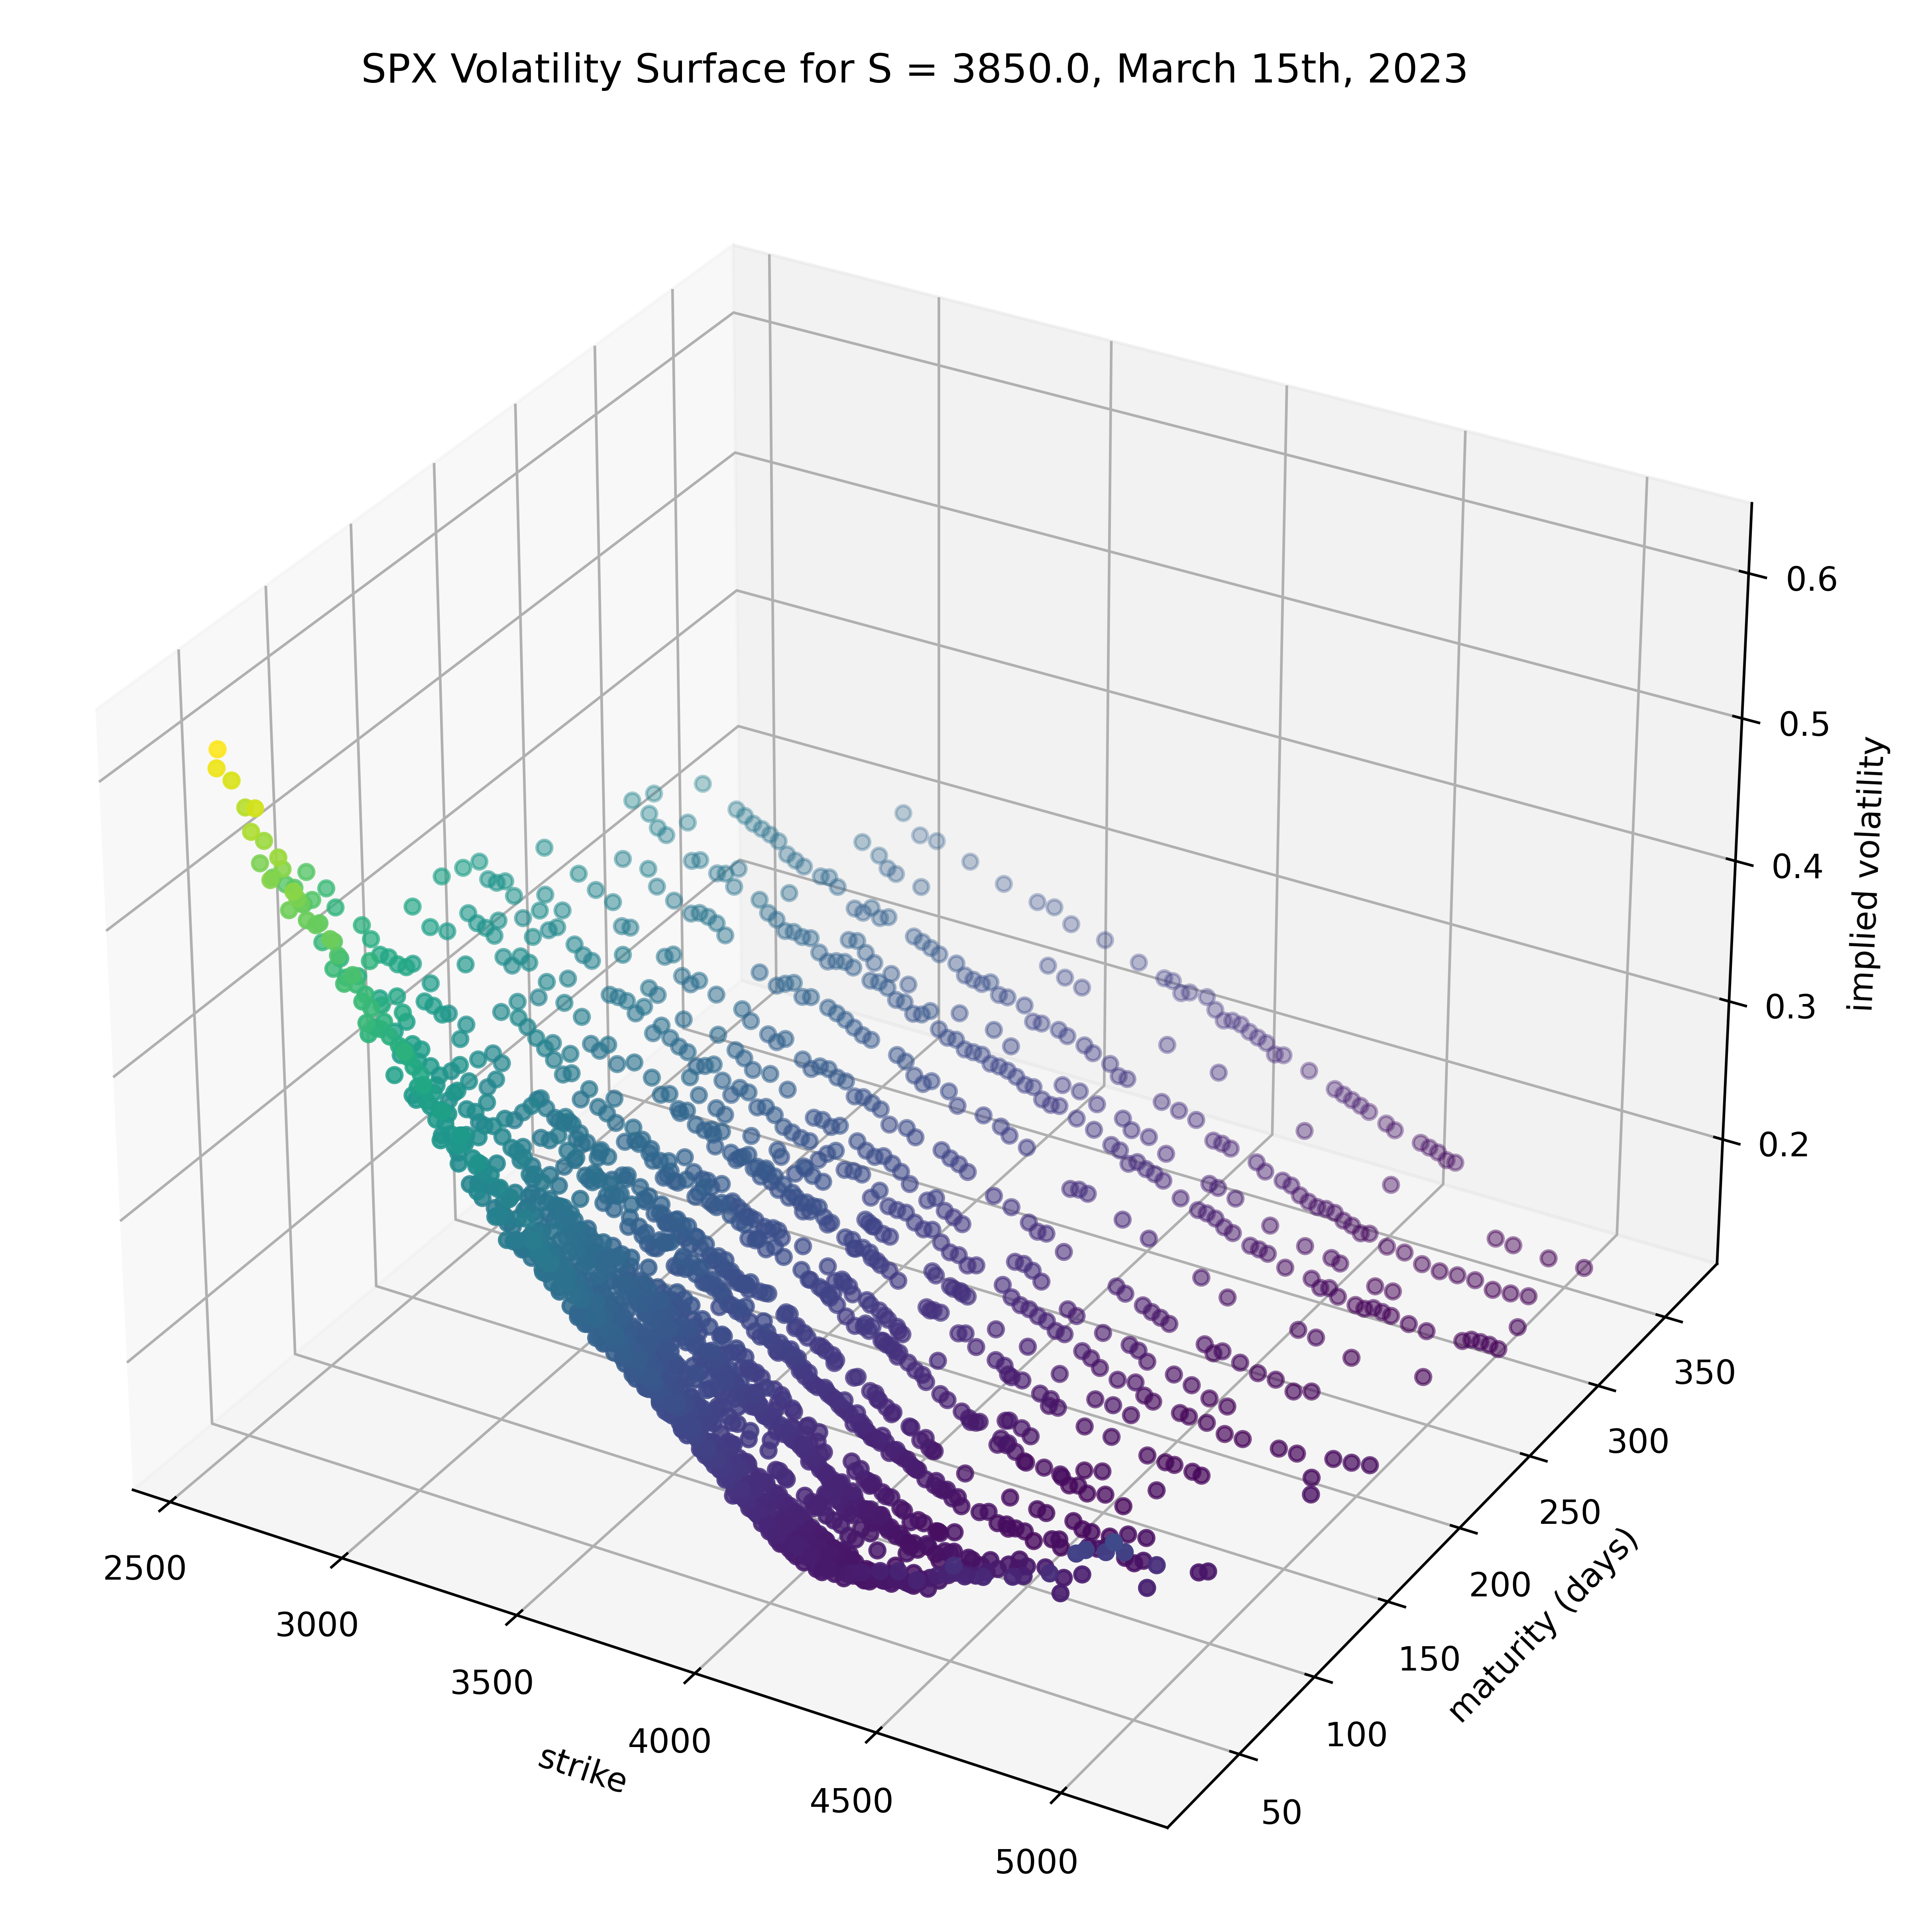
\includegraphics[width=\textwidth]{surface.png}
	\caption{Illustrative set of implied volatilities extracted from one day of SPX options trade data}
	\label{fig:surface}
\end{figure}
\newpage
\subsection{Distribution of market parameters}
\begin{figure}[h!]
	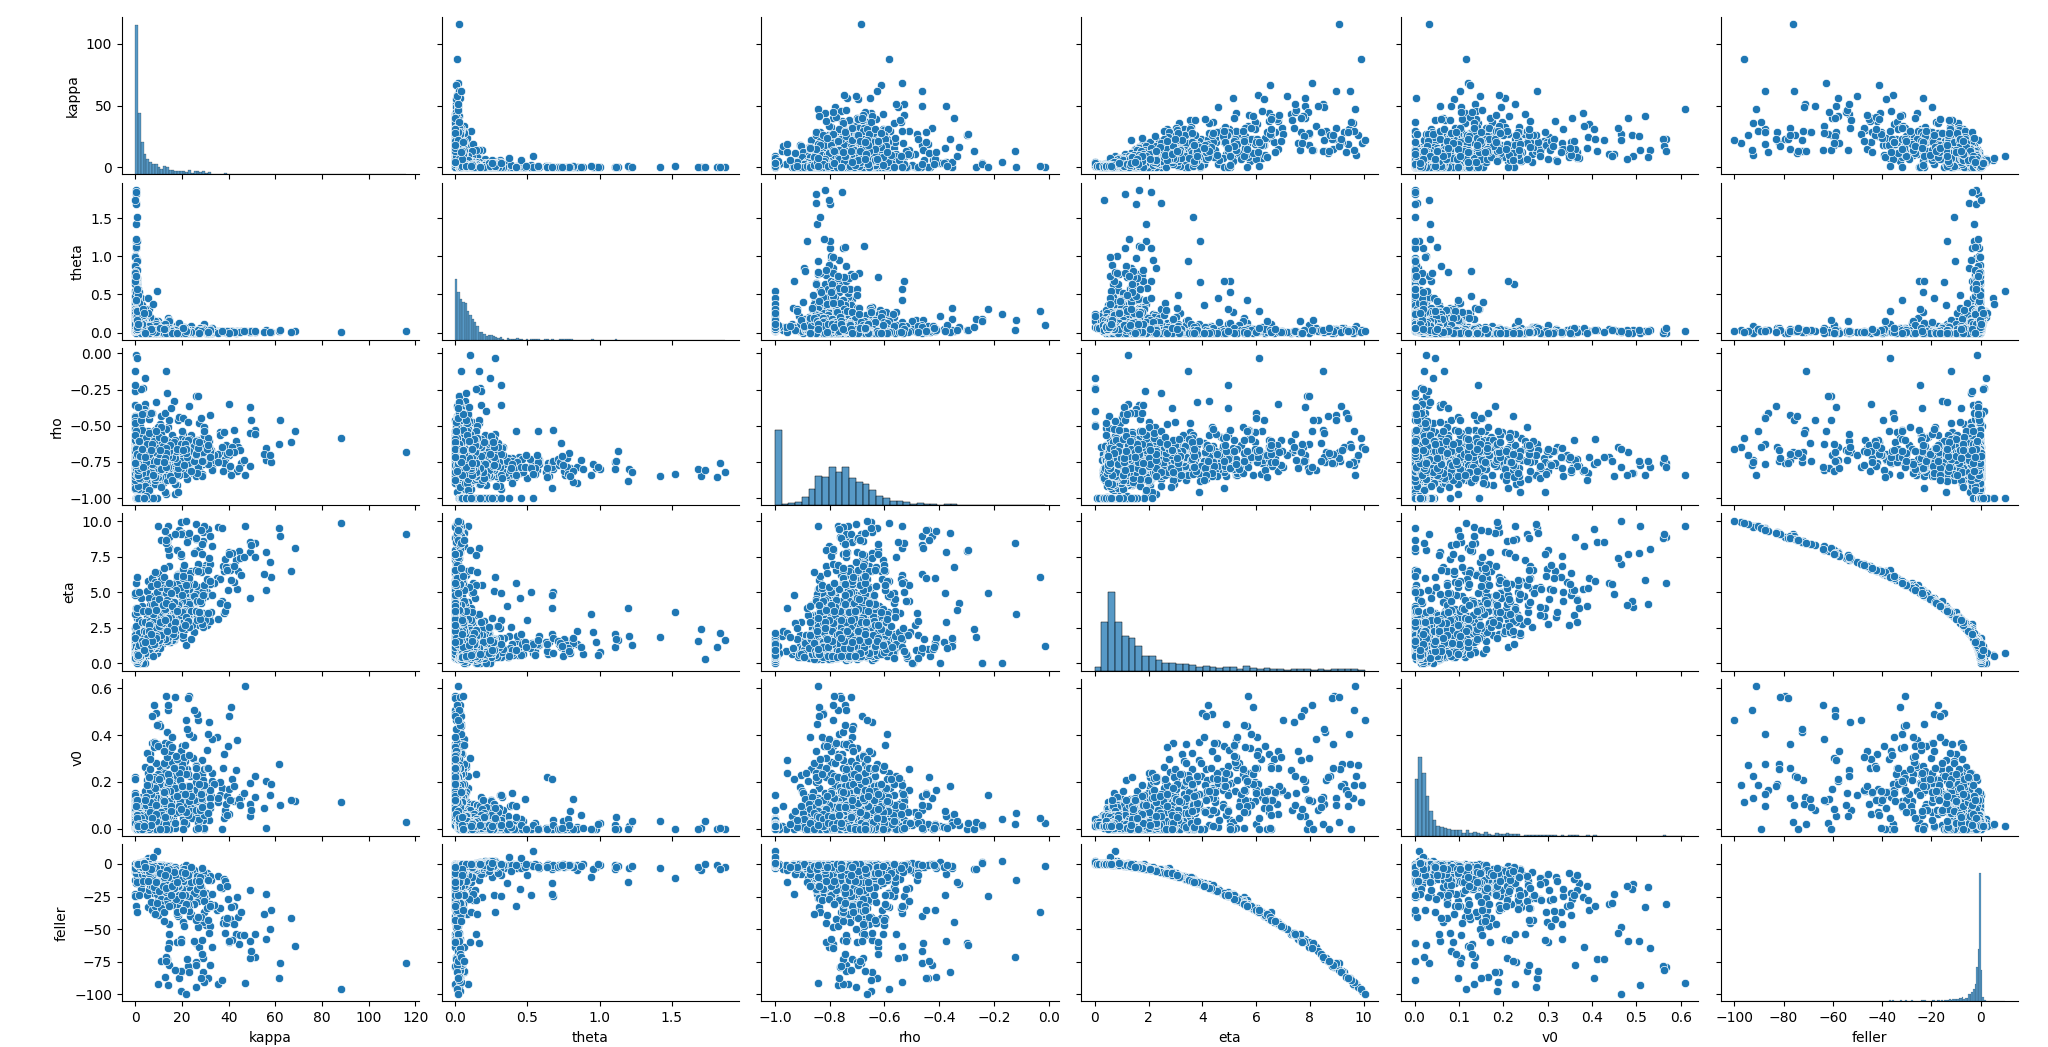
\includegraphics[width=0.98\textwidth]{market.png}
	\caption{Distribution of Heston~\cite{heston_1993_a} pricing model parameters}
	\label{fig:market}
\end{figure}